\section{Experiment with Pozyx}\label{sprint1:experiment}
To determine the accuracy of the Pozyx tags an experiment was conducted.
The primary goal of the experiment was to test the accuracy, but a secondary goal of the experiment was to determine the frequencies of updates for each tag.
\\
\subsection{Purpose}
According to research regarding latency in VR \cite{WaltemateThomas2016Tiol} and interactive systems \cite{10.1145/169059.169431}, the number of movement errors increase as the latency increases.
An example of this is when a tag is moved, and the tag first sends a new position after 3 seconds, then the movement error could be high as the user does not know their exact position for these 3 seconds.
According to experiments with VR, the motor performance and sense of body ownership start to decrease at latencies above 75 ms.\\
This means that the optimal results from these experiments would indicate that the Pozyx system can send position updates fast enough which allows the system to operate with a latency of less than 75 ms between their physical movement and the in-game reflection of this movement.

\subsection{Setup}
The tags were set to transmit with the highest bitrate with the longest preamble length and with the ranging mode set to precise \cite{pozyx-Performance}.\\
According to the documentation, these values lower the tags update rate to about 9hz which is then divided by the number of tags used in the system as described in \autoref{pozyx:TWR}.
As the main goal of the experiment was to test the accuracy these settings were chosen to gives the most accurate positioning.
The settings can be changed at a later point to try to increase the update rate to a level where the latency for the users is acceptable.\\
The experiment was set up as shown on \autoref{fig:experiment-setup}.
The experiment was conducted indoors on our campus in the building Novi 9.
The anchors \texttt{0x632b} and \texttt{0x676e} were mounted on a wall 240 centimeters apart, and the remaining anchors \texttt{0x6738} and \texttt{0x676c} were mounted on a bulletin board.\\
The number of centimeters accompanying the hexadecimal number of each anchor is the height at which the anchor was mounted during the experiment.
Different heights were chosen as Pozyx documentation suggests that not all anchors should have the same height \cite{pozyx-AnchorHeights}.
The reason for this is the principle of geometric dilution of precision (GDOP), which can cause the error on range measurements to be amplified.

\begin{figure}[H]
    \centering
    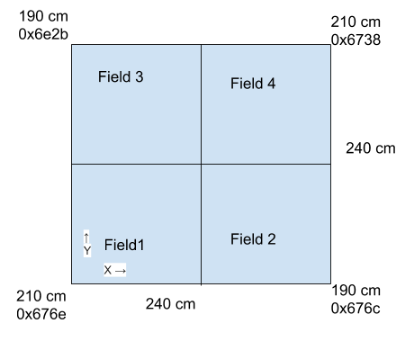
\includegraphics[width=0.6\linewidth]{experiment-setup.PNG}
    \caption{The setup of the experiment with the anchors and the height at which they were placed in the corners. The hexadecimal number is the anchor, and above that is the height at which the anchors were placed.}
    \label{fig:experiment-setup}
\end{figure}
\noindent
The fields were created by a whiteboard on which lines were drawn every 10 centimeters to know the actual position as seen on \autoref{fig:experiment-blackboard}.
This whiteboard was moved intermittently to act as respectively fields 1, 2, 3, and 4.

\begin{figure}[H]
    \centering
    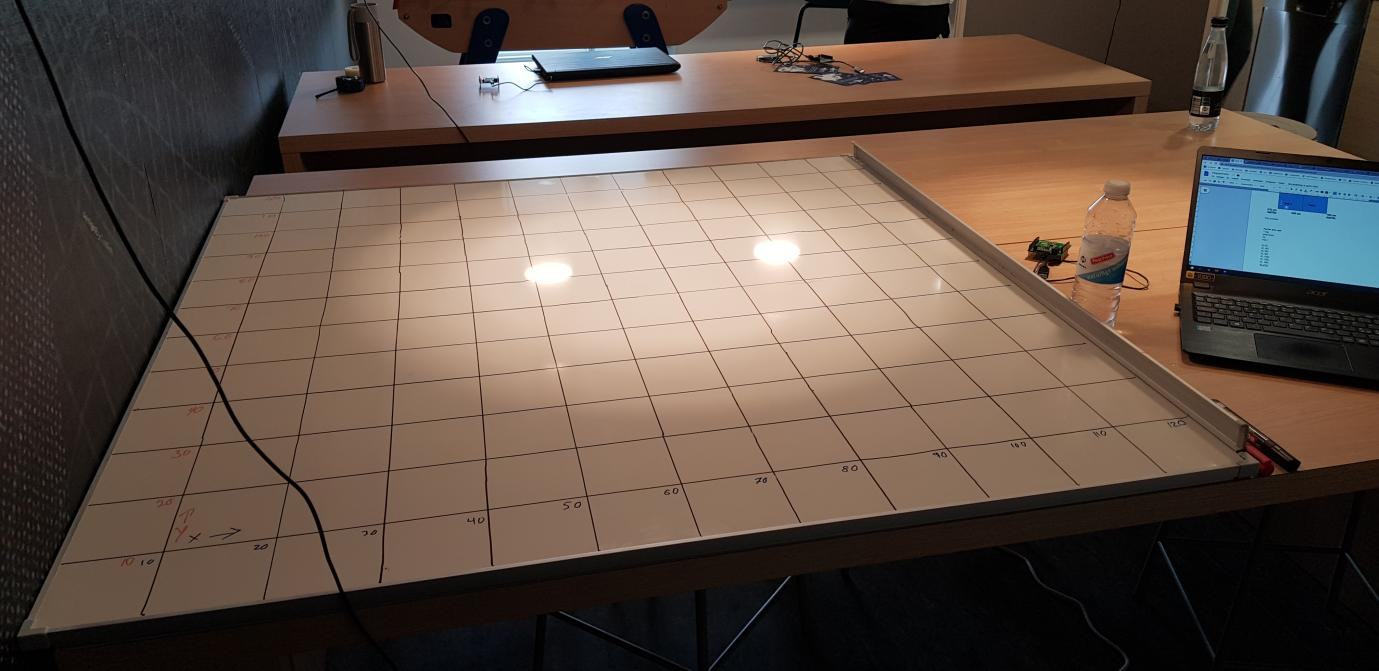
\includegraphics[width=0.8\linewidth]{experiment-blackboard.png}
    \caption{The whiteboard with the drawn positions.}
    \label{fig:experiment-blackboard}
\end{figure}
\noindent
The procedure for the experiment was based on this whiteboard.
The whiteboard would be placed in one of the fields defined in \autoref{fig:experiment-setup}, and the tags would be placed in certain positions on the board and record the accuracy with which the position was reported.
The tags would be placed in a position, remain there for five seconds, then be moved to the next position over the next five seconds and remain in this position for five seconds before being moved again.
This procedure was repeated until a satisfactory number of measurements had been made.
This amount was usually 5 measurements.
Once one field had been tested, the whiteboard was moved to the next field, as seen on \autoref{fig:experiment-setup}, and the process was repeated.

\subsection{Analyzing the data}
In \autoref{app:experiment} the data for the experiment can be seen.
For each test the average grid was calculated, and the minimum and maximum values for $x$, $y$ and $z$ were found.
The min and max values were noted, as they may be useful for future analysis.
The $z$ values were very inconsistent throughout the entire test, and due to this and the $z$-axis being largely irrelevant to the game, we will not focus on analyzing them.
Because of this, it was decided to only calculate the deviance between the actual position and the measured position in the $xy$-plane.

\subsubsection{Precision with 1 tag}
When testing with only one tag the average of all deviations was 15.20 cm.
\begin{figure}[H]
    \centering
    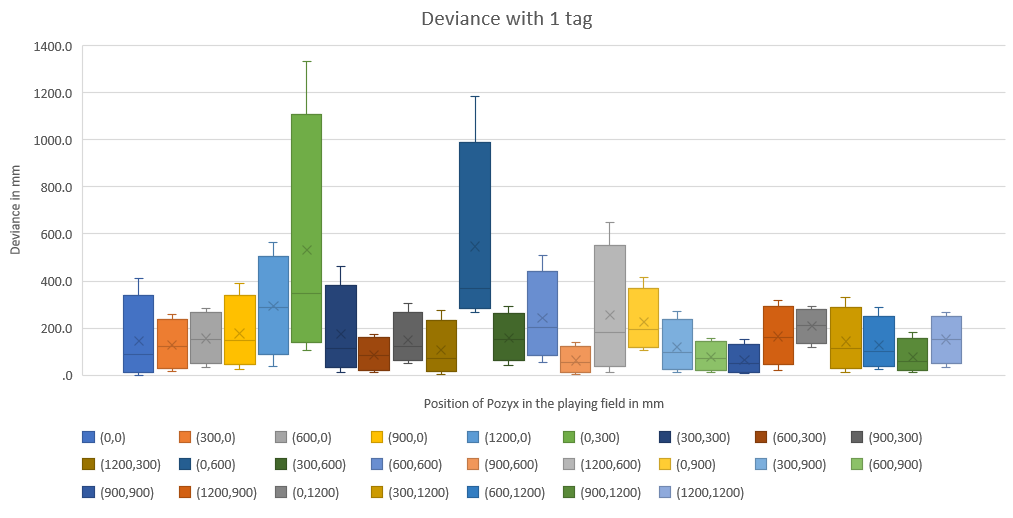
\includegraphics[width=1\linewidth]{1tagdiagram.PNG}
    \caption{A box plot showing the dispersion of measured positions with 1 tag}
    \label{fig:1tagdiagram}
\end{figure}
\noindent
As can be seen on \autoref{fig:1tagdiagram}, some measurements can be quite far off the actual position.
On the $x$-axis you can see the actual position of the tag in mm compared to the playing field.
The $y$-axis shows the amount that the measurements were off the actual position in mm.
Each measurement set has its own box and whiskers.
The box shows the measurements within the first quartile and third quartile.
Within the box the $X$ denotes the second quartile which is equal to the median and the flat line denotes the average value of all the measurements.
Extending from the box is the lower and upper whiskers where the lower whisker shows the measurements below the first quartile and the upper whisker shows the measurements above the third quartile.
The end of the lower whisker is the lowest deviance measured in the set, likewise the end of the upper whisker is the highest deviance measured.

Interestingly it is the measurements closest to the $x$-axis that are the most inaccurate, we will discuss why in \autoref{subsec:influence-on-the-test}.
The measurement with the highest deviance was recorded when the tag was in position \texttt{(0,3000)} where the measured position was 1.3 meters off.
The average deviance of all the measurements from that position was only 36.5 cm, however.
The highest average deviance of all the positions was 39.5 cm in position \texttt{(0,6000)}.
When running with one tag the average amount of measurements were 12.368 per second.


\subsubsection{Precision with 3 tag}
For this part of the experiment, the accuracy was tested with three tags.
The tags were positioned at three different x-coordinates.
1400, 1800 and 2200 were chosen as the $x$ coordinates and the $y$ coordinate was moved up by 300 mm each time starting from 0 and going up to 1200.
The average amount of updates from all the tags per second were 1.83, less than 10 percent of the amount of updates when only one tag was used.
The amount of updates were very different between the different tags, as the one with the highest update rate had an average of 3.4 per second and the lowest only 0.92.
\begin{figure}[H]
    \centering
    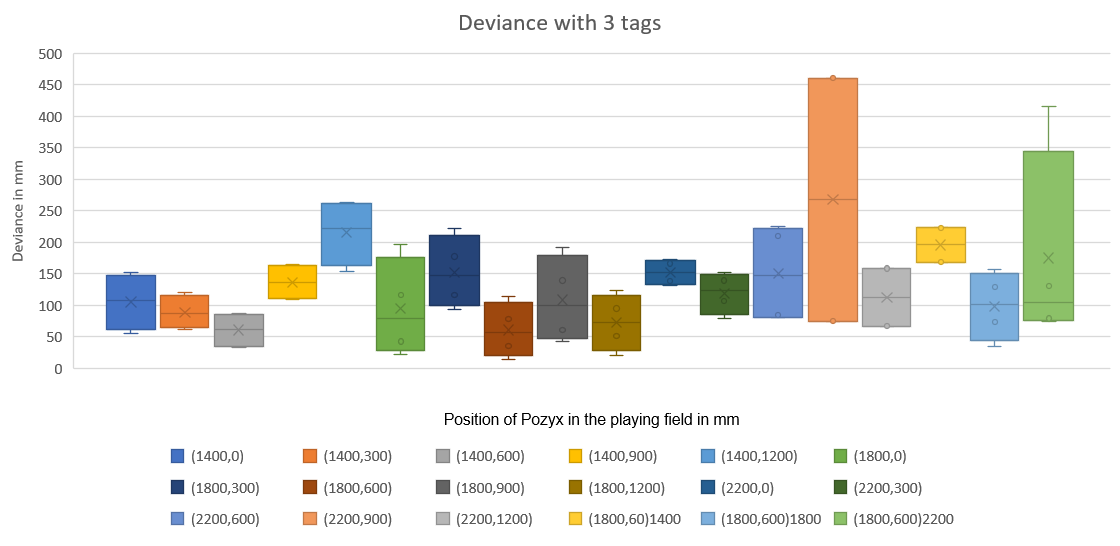
\includegraphics[width=1\linewidth]{3tagdiagram.PNG}
    \caption{A box plot showing the dispersion of measured positions with 3 tags}
    \label{fig:3tagdiagram}
\end{figure}
\noindent
On \autoref{fig:3tagdiagram} all the measurements from the 3 tag experiment can be seen.
The 3 last sets of measurements are from when all the tags were placed close to each other at the same point.
The trailing number after the coordinate is which tag the set of measurements belong to, \texttt{(1800,600)1400} denotes the tag used for the measurments along the line where $x$ equals 1400.

This was done to see if they would affect the precision of each other.
Based on the data it seems they might have a small effect on each other but not enough for it to be a problem.
The biggest deviance in the test was only 46 cm off compared to 1.3 meters in the 1 tag test which seemed interesting, but could be because the measurements in the 3 tag experiment were made in the middle of the playing field compared to at the edge in the 1 tag experiment.

\paragraph{Tag 0x6763}
This tag was positioned 1400 mm along the $x$-axis.
The overall average deviation for this tag was 11.9 cm and it made 1.16 measurements per second.
No measurements were further away than 26.3 cm from the actual position and the biggest average deviance for a set of measurements was only 22.26 cm.


\paragraph{Tag 0x690F}
This tag was positioned 1800 mm along the $x$-axis.
This tag was only 9.2 cm off on average and had by far the highest average update rate at 3.4 Hz.
Like the previous tag it also did not have any measurements with large deviances.
The furthest measurement was 22.1 cm off and the worst average deviance for a set was 15.09 cm.
This was by far the best performing tag in this experiment regarding both precision and update rate.

\paragraph{Tag 0x602E}
This tag was positioned 2200 mm along the $x$-axis.
The overall average deviation for this tag was 14.48 cm and an update rate at 0.92 hz.
For the first three points the results seemed fairly accurate, however, the grid \texttt{(2200, 900)} had a large deviation of 22.43 cm.
That set also had the measurement with highest deviance with 46.0 cm.

\subsubsection{Precision with 5 tag}
The tags were positioned at five different x-coordinates.
1400, 1600, 1800, 2000 and 2200 were chosen as the $x$ coordinates and the $y$ coordinate was moved up by 200 mm each time starting from 0 to 1200 mm.
\begin{figure}[H]
    \centering
    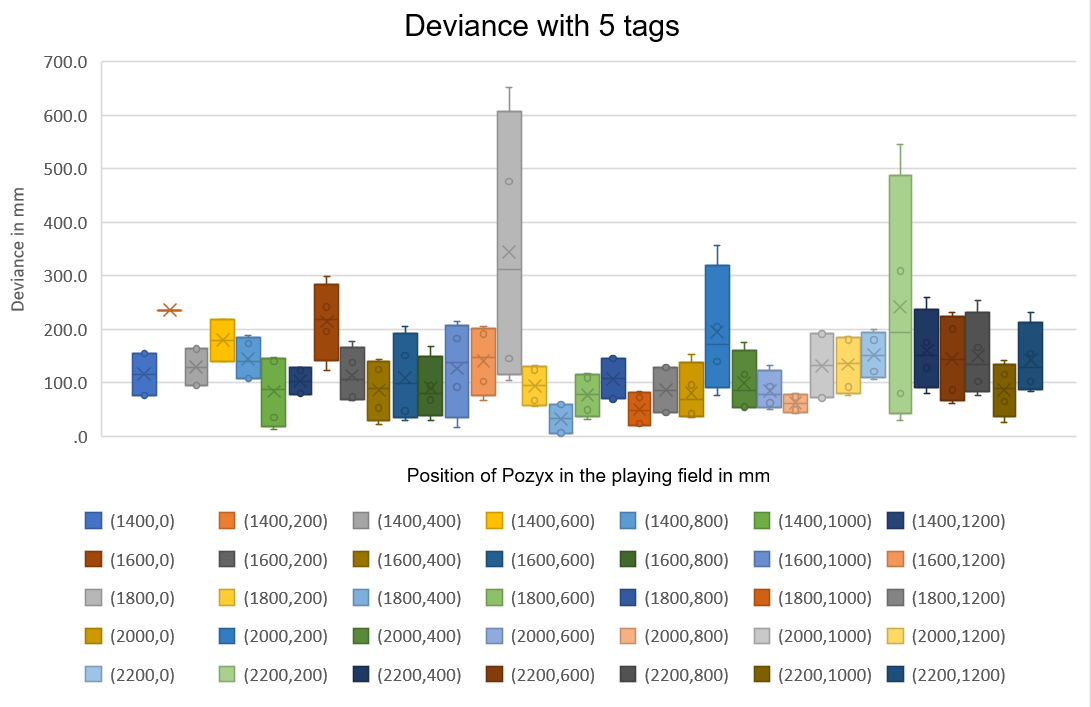
\includegraphics[width=1\linewidth]{5tagdiagram.PNG}
    \caption{A box plot showing the dispersion of measured positions with 5 tags}
    \label{fig:5tagdiagram}
\end{figure}
\noindent
Like the experiment with 3 tags, seen on \autoref{fig:3tagdiagram}, there were no huge outliers like in the first experiment where some measurements were off by more than a meter.
But two instances were still seen as further off than the average.


\paragraph{Tag 0x602E}
This tag was positioned 1800 mm along the $x$-axis.
The average deviation for this tag was 12.99 cm and the average update rate was 0.83 Hz.
This was the tag that had the worst measurement on coordinates \texttt{(1800, 0)} which was off by 65.1 cm and the worst average deviance of a measurement set with 31.7 cm.
Besides that the other sets were among the most accurate.

\paragraph{Tag 0x6763}
This tag was positioned 1400 mm along the $x$-axis.
For this tag, the average deviation was 12.75 cm and the average amount of data points per second was 0.6.
At \texttt{1400, 200} the tag only returned one measurement and at \texttt{(1400, 600)} there were only two measurements completed during the 5 second period the tag was in that position.
The tag was overall very precise with all measurements within 23.6 cm of the actual position.

\paragraph{Tag 0x690F}
This tag was positioned 1600 mm along the $x$-axis.
Tag 0x690F had an average deviation of 12.39 cm and an update rate at 2.11 Hz.
This update rate was much higher than tag 0x602E, 0x6763 and 0x6979, and equal to 0x6915 even though they all had the same settings.

\paragraph{Tag 0x6915}
This tag was positioned 2200 mm along the $x$-axis.
The average deviation of tag 0x6915 was 14.74 cm, and it had an update rate of 2.11 Hz aswell.
This tag had a few spikes when measuring on coordinate \texttt{(2200, 200)}, where the average deviance was 20.99 cm and the worst measurement was 54.6 cm off.

\paragraph{Tag 0x6979}
This tag was positioned 2000 mm along the $x$-axis.
The average deviation of this tag was 10.46 cm and the average update rate was 1.23 Hz.
This tag was pretty average with no big deviations.
Its worst measurement set had an average deviation of 18.34 cm.


\subsection{Possible influences on the test}\label{subsec:influence-on-the-test}
One thing that could have affected the tags is that a whiteboard was used as a measure for positions.
As there is metal in the whiteboard this could have affected the precision of the tags.
Metals are conductors, which can lead to the signal having less power and reduced range, and the signal might spend extra time trying to get through the metal.
Since Pozyx positioning relies on calculating the time of flight, having the signal spend extra time traveling reduces accuracy \cite{pozyx-UWBObstacles}.
\\\\
If we look at the $z$ coordinate in the test experiment data, it can be seen that $z$ fluctuates a lot more than the $x$ and $y$ coordinates.
The max $z$ coordinate for multiple experiments is often more than 3 meters and the average $z$ coordinate is also often 1 meter higher than the actual coordinate.
This could be due to the height difference between the anchors not being sufficiently large which can affect Pozyx' ability to measure the height of the tags.
\\\\
During the test with 1 tag, the 0 value of the $x$ coordinate coincided with the wall.
This could have been an influence on the positioning result in that it could increase uncertainty, as it was difficult to center the tag over the x coordinate since the coordinate collided with the wall.
Also, the wall could have created interference with the signal and there might have been metal or wires going through it which could have affected the signal.
\\\\
While the experiment was running the tags could throw errors instead of giving a position if something went wrong.
Mainly during the multi-tag tests, some tags would report back with errors such as unable to get firmware version, flash memory corrupted or an error message saying there was no error.
At that point in the experiment, it was not clear whether it was a hardware error with some of the tags or if it was code related.
The tags would throw these errors randomly and then measure their position normally at the next update.
This resulted in some of the tags having periods of update rates of less than 0.2 Hz.
It was decided that further investigation into this issue should be conducted at a later point.

\subsection{Conclusion on the experiment}
Our conclusion of this experiment is that the precision is satisfactory, but the update rate is not optimal as that does not meet the standards of the refresh rate needed with the current settings.
\\\\
We also need to consider the spikes in the coordinates, such that the user does not jump around on the screen, even though the user might not be moving.
A good solution would be to use an algorithm to correct the data.
\\\\
The results of this experiment shows that a three dimensional game is not viable with the errors that we had on the $z$ coordinate.
This is most likely due to the height difference between the anchors only being 20 cm.
If we, later on, choose to make use of the $z$ coordinate, then it is necessary to conduct another experiment with the Pozyx with different, larger height differences, but as it currently is only a two-dimensional game it is not necessary.
\\\\
It also seemed like some tags were not able to send as many measurements as others.
Consistently throughout the experiments tag 0x690F was the best tag regarding update rate, sometimes having an update rate almost 3 times faster than the other tags.
This was caused in part due to some tags seemingly having a slower update rate, but also because some of them would report errors instead of measurements randomly.
This is something that will be investigated.
